\subsection{Shape Analysis}

This appendix shows the kinematic variables and the BDT output
for the BDT analysis selection in the 0 and 1-jet bins.
The variables are shown inclusively of the BDT output,
as well as for low BDT score and high BDT score.
The mass hypothesis $125\GeV$ is shown in Figures \ref{fig:hww_kinematics_125_0j} to \ref{fig:hww_bdthi_kinematics_125_1j}.
The mass hypothesis $160\GeV$ is shown in Figures \ref{fig:hww_kinematics_160_0j} to \ref{fig:hww_bdthi_kinematics_160_1j}.
The mass hypothesis $200\GeV$ is shown in Figures \ref{fig:hww_kinematics_200_0j} to \ref{fig:hww_bdthi_kinematics_200_1j}.

\clearpage
%%%%%%%%%%%%%%
\begin{figure}[!htp]
\centering
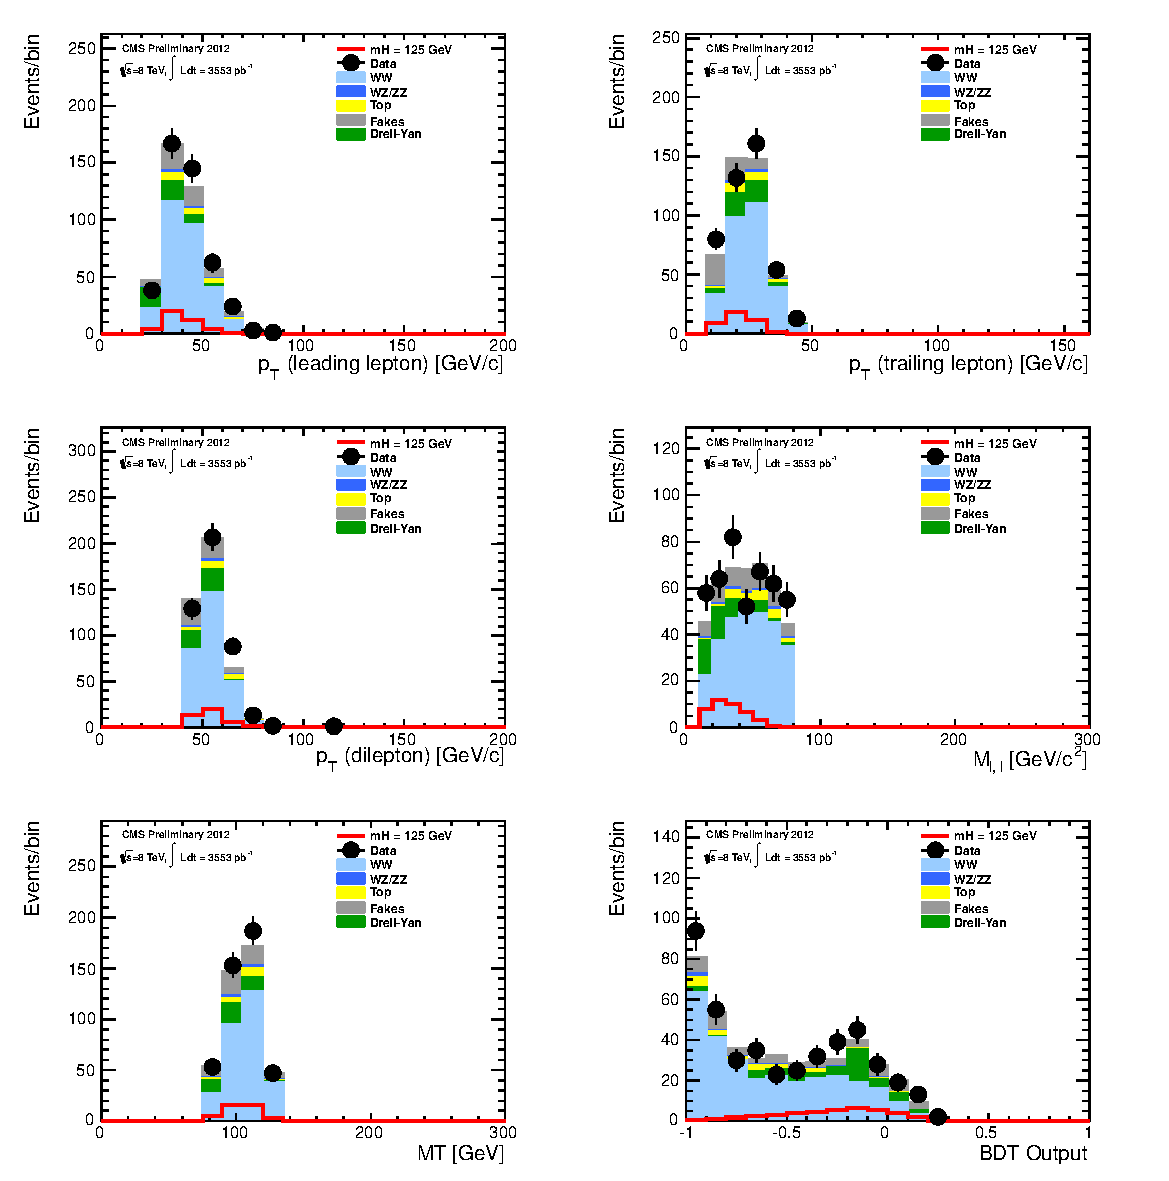
\includegraphics[width=1.0\textwidth]{figures/hww_analysis18_125_ALL_incl_0j.pdf}
\caption{Kinematic distributions in the 0-jet bin for $m_{H}=125\GeV$.}
\label{fig:hww_kinematics_125_0j}
\end{figure}
\begin{figure}[!htp]
\centering
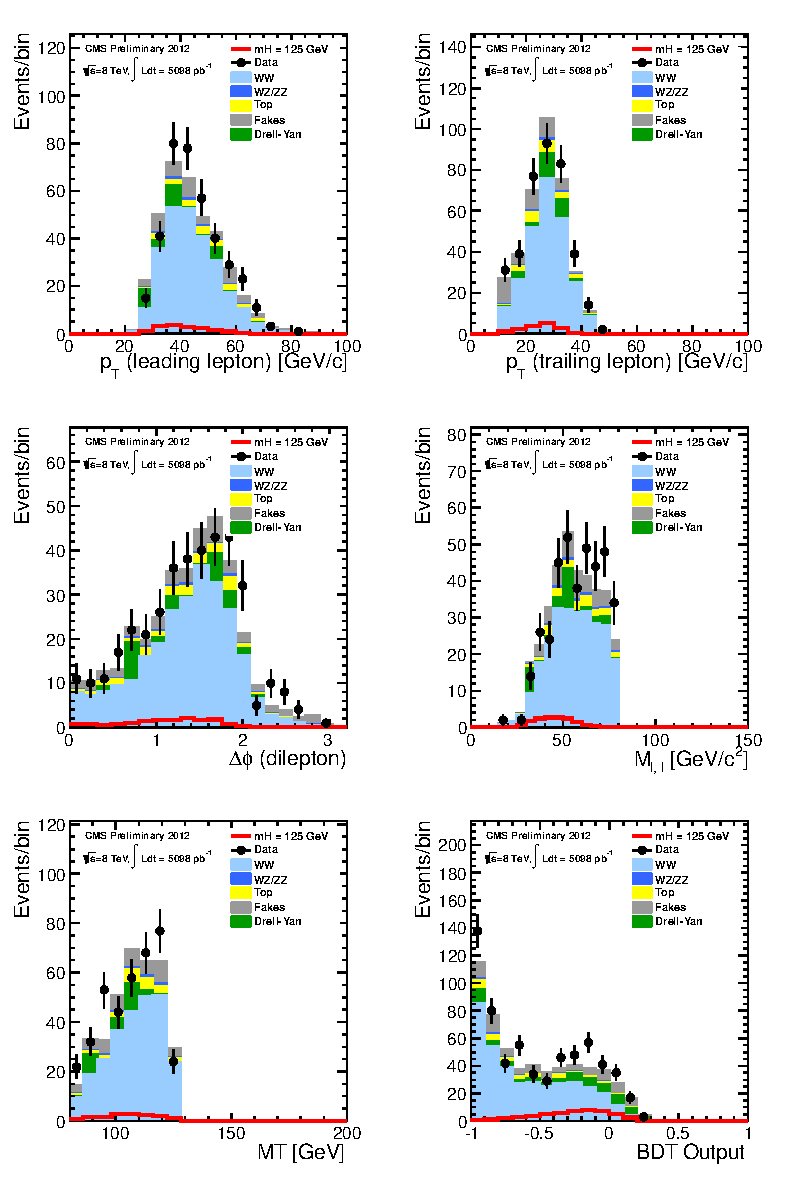
\includegraphics[width=1.0\textwidth]{figures/hww_bdtlo_analysis18_125_ALL_incl_0j.pdf}
\caption{Kinematic distributions in the 0-jet bin for $m_{H}=125\GeV$ (BDT$< -0.4$).}
\label{fig:hww_bdtlo_kinematics_125_0j}
\end{figure}
\begin{figure}[!htp]
\centering
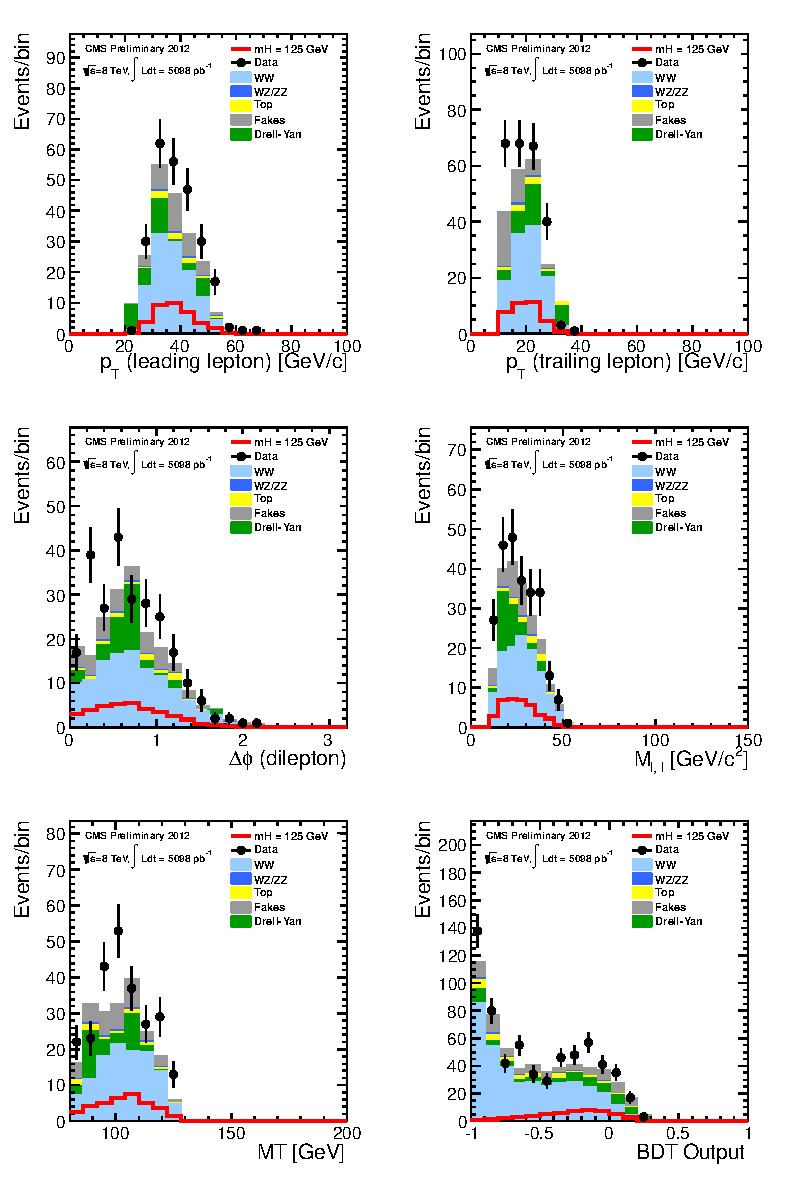
\includegraphics[width=1.0\textwidth]{figures/hww_bdthi_analysis18_125_ALL_incl_0j.pdf}
\caption{Kinematic distributions in the 0-jet bin for $m_{H}=125\GeV$ (BDT$> -0.4$).}
\label{fig:hww_bdthi_kinematics_125_0j}
\end{figure}
\begin{figure}[!htp]
\centering
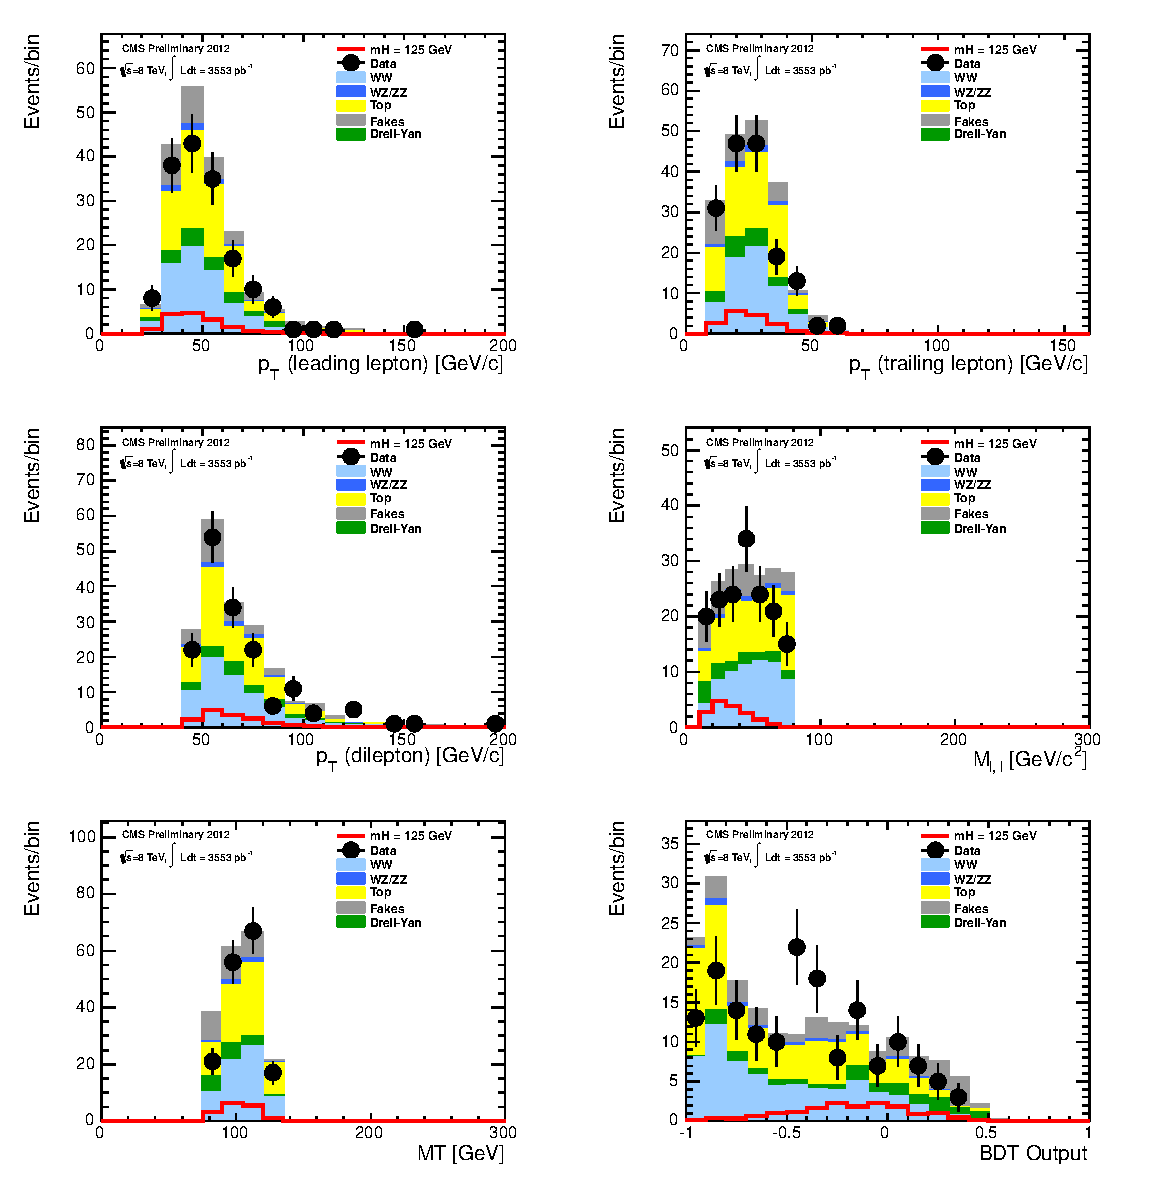
\includegraphics[width=1.0\textwidth]{figures/hww_analysis18_125_ALL_incl_1j.pdf}
\caption{Kinematic distributions in the 1-jet bin for $m_{H}=125\GeV$.}
\label{fig:hww_kinematics_125_1j}
\end{figure}
\begin{figure}[!htp]
\centering
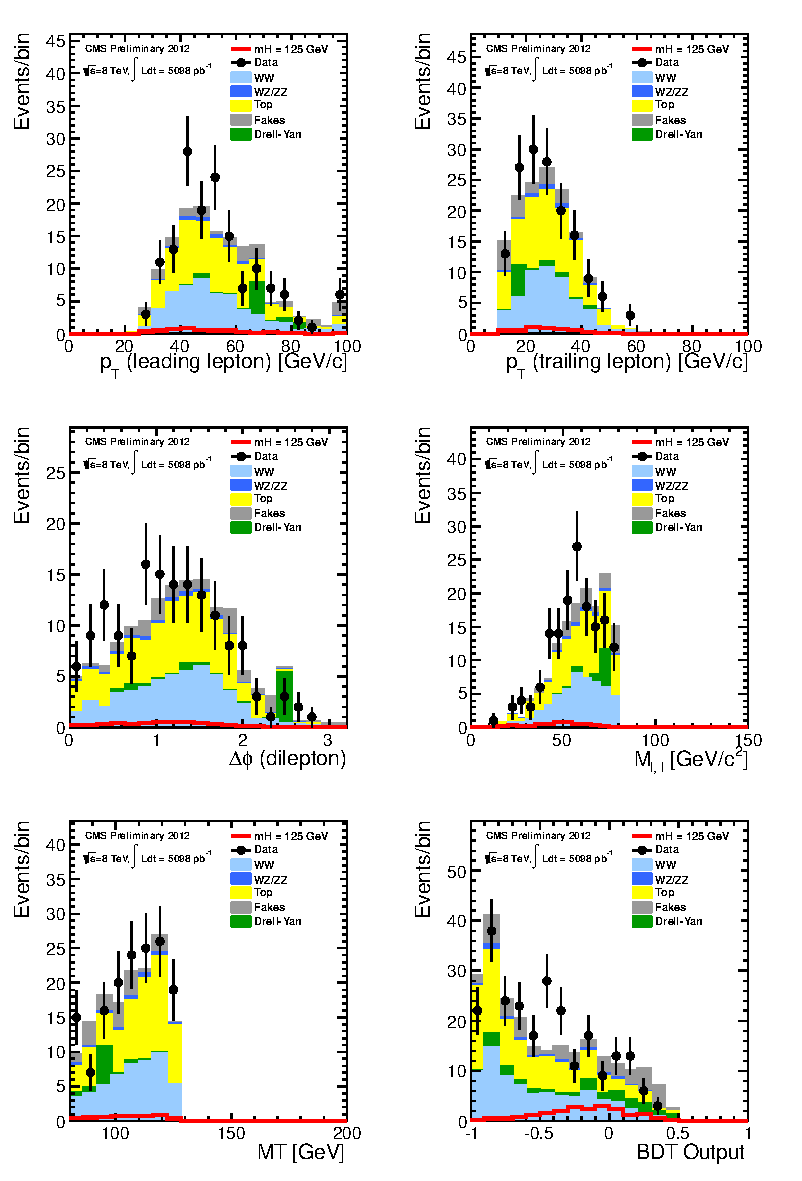
\includegraphics[width=1.0\textwidth]{figures/hww_bdtlo_analysis18_125_ALL_incl_1j.pdf}
\caption{Kinematic distributions in the 1-jet bin for $m_{H}=125\GeV$ (BDT$< -0.4$).}
\label{fig:hww_bdtlo_kinematics_125_1j}
\end{figure}
\begin{figure}[!htp]
\centering
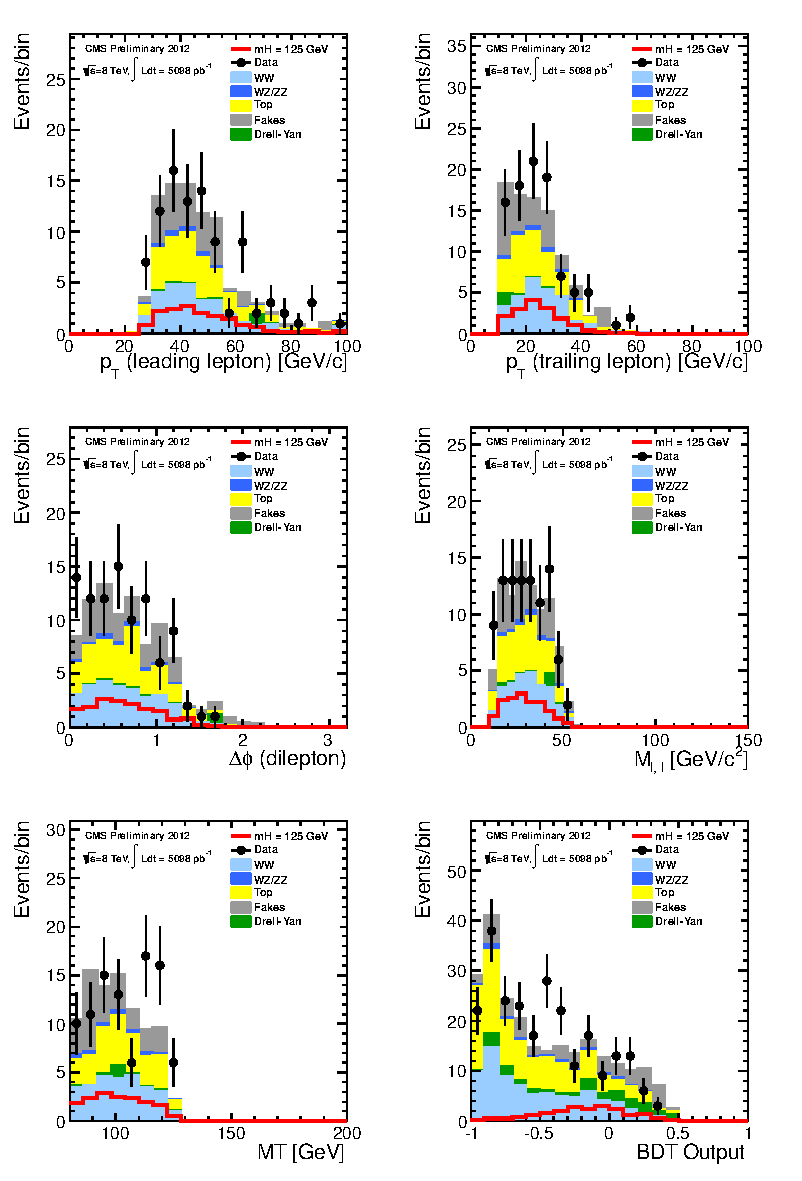
\includegraphics[width=1.0\textwidth]{figures/hww_bdthi_analysis18_125_ALL_incl_1j.pdf}
\caption{Kinematic distributions in the 1-jet bin for $m_{H}=125\GeV$ (BDT$> -0.4$).}
\label{fig:hww_bdthi_kinematics_125_1j}
\end{figure}
%%%%%%%%%%%%%%
\clearpage
%%%%%%%%%%%%%%
\begin{figure}[!htp]
\centering
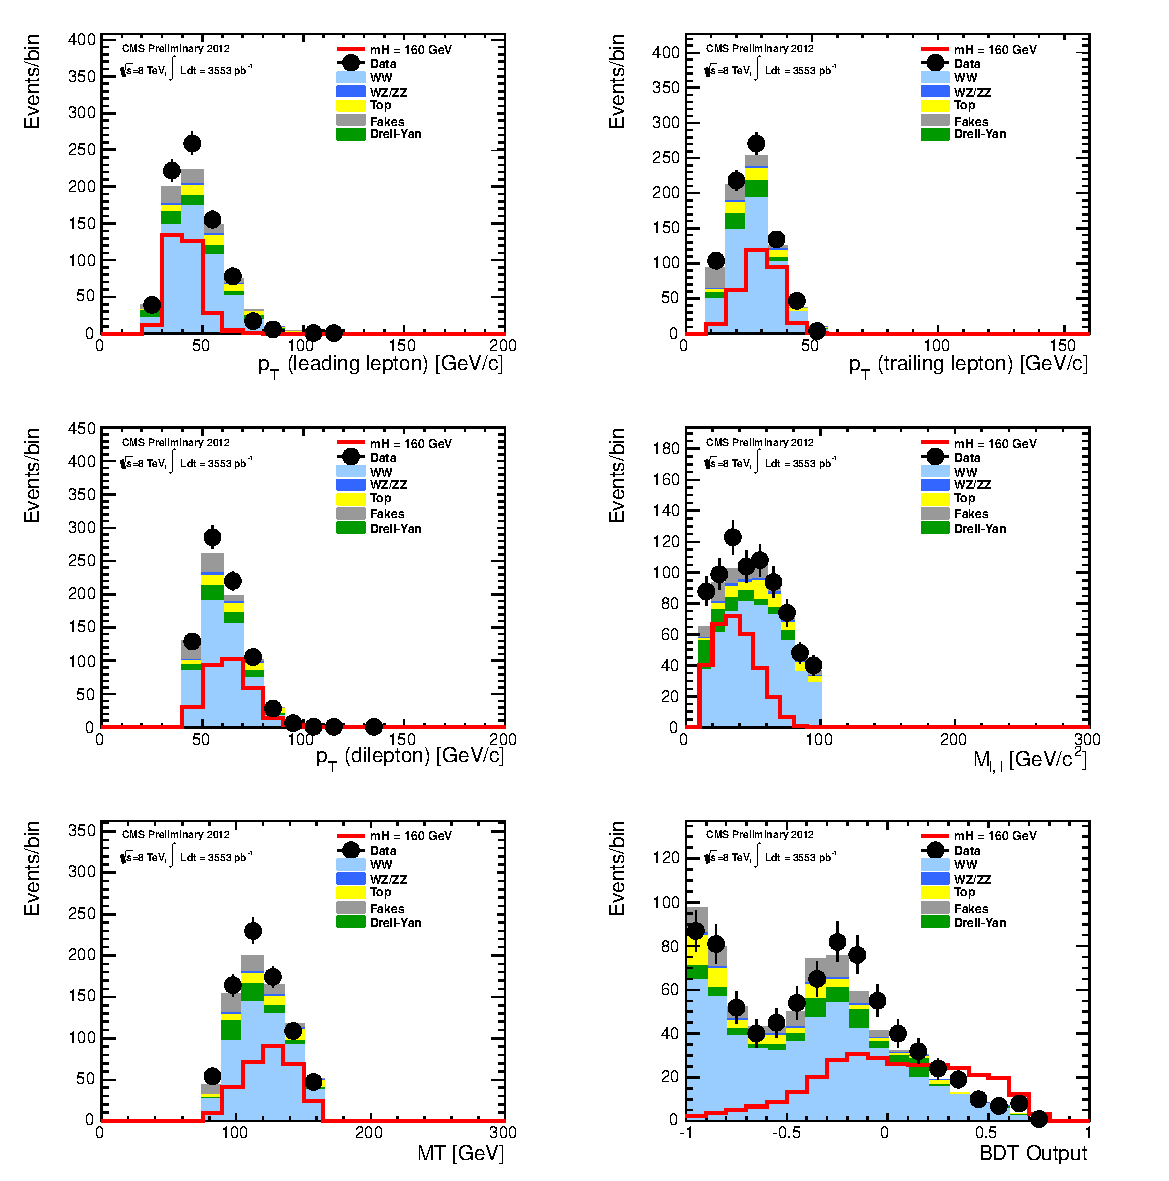
\includegraphics[width=1.0\textwidth]{figures/hww_analysis18_160_ALL_incl_0j.pdf}
\caption{Kinematic distributions in the 0-jet bin for $m_{H}=160\GeV$.}
\label{fig:hww_kinematics_160_0j}
\end{figure}
\begin{figure}[!htp]
\centering
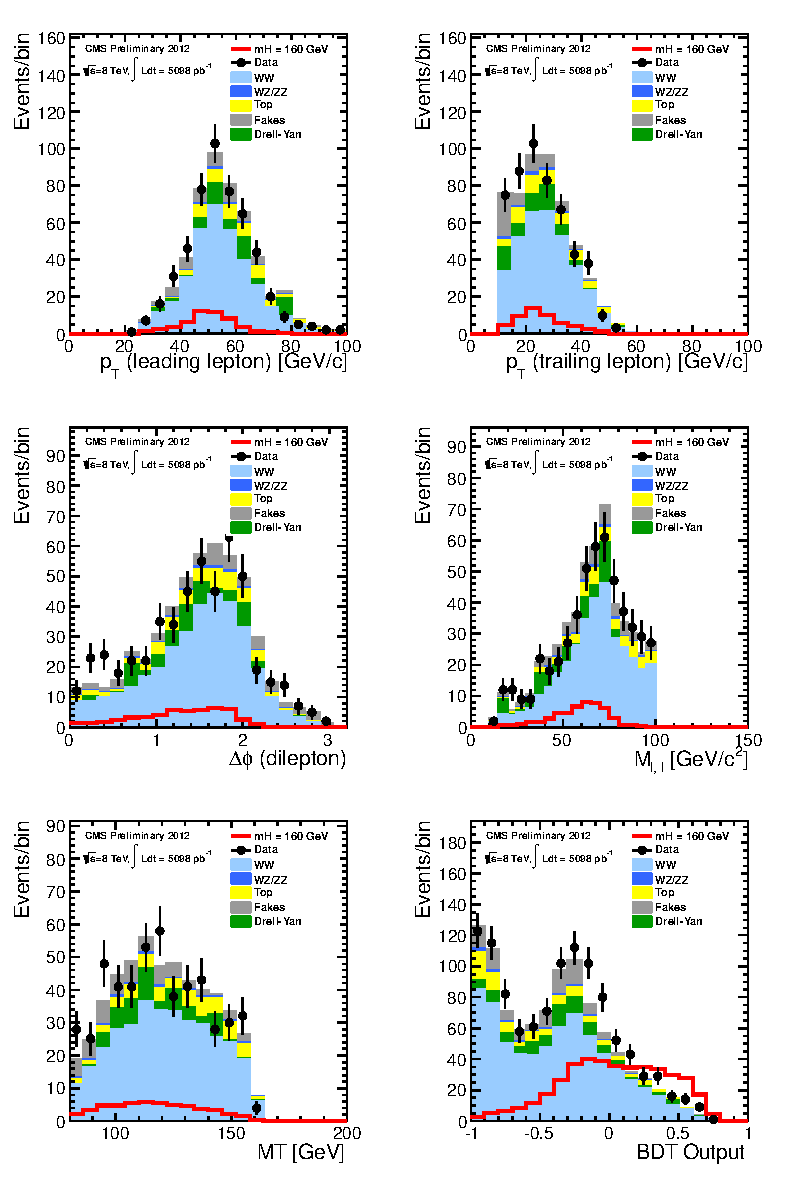
\includegraphics[width=1.0\textwidth]{figures/hww_bdtlo_analysis18_160_ALL_incl_0j.pdf}
\caption{Kinematic distributions in the 0-jet bin for $m_{H}=160\GeV$ (BDT$< -0.4$).}
\label{fig:hww_bdtlo_kinematics_160_0j}
\end{figure}
\begin{figure}[!htp]
\centering
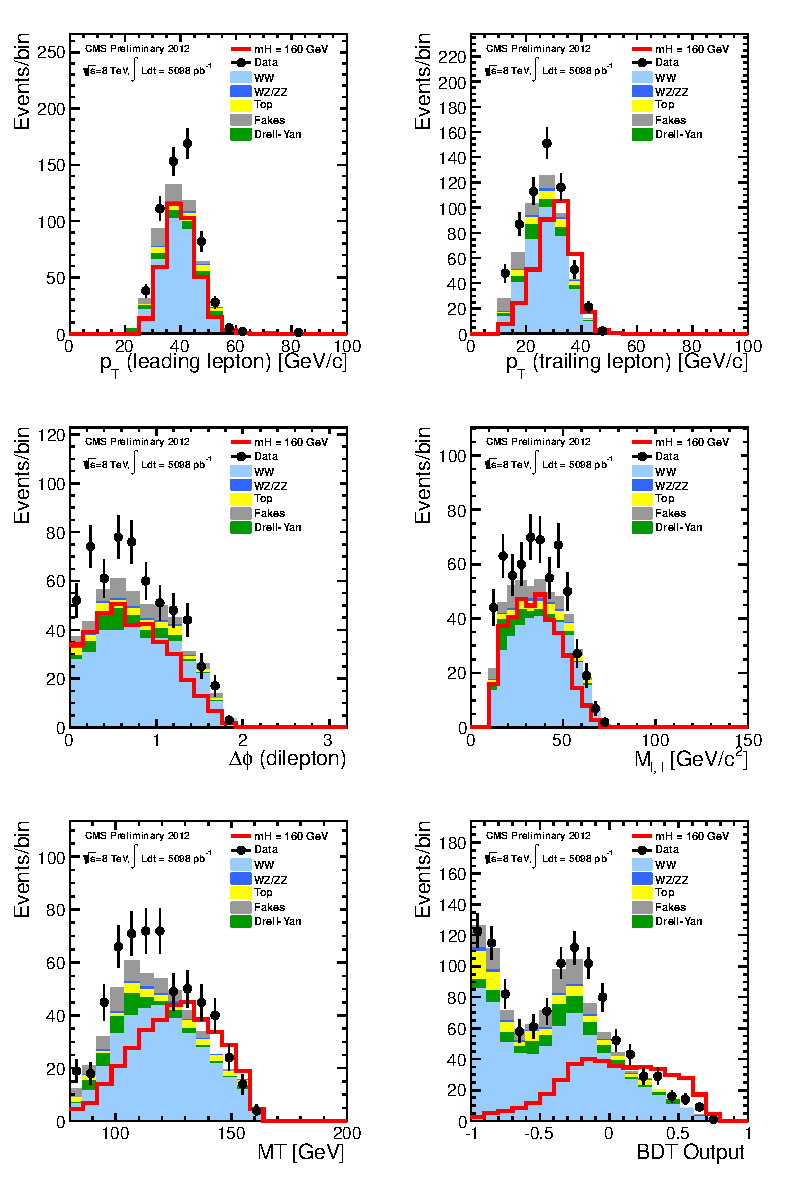
\includegraphics[width=1.0\textwidth]{figures/hww_bdthi_analysis18_160_ALL_incl_0j.pdf}
\caption{Kinematic distributions in the 0-jet bin for $m_{H}=160\GeV$ (BDT$> -0.4$).}
\label{fig:hww_bdthi_kinematics_160_0j}
\end{figure}
\begin{figure}[!htp]
\centering
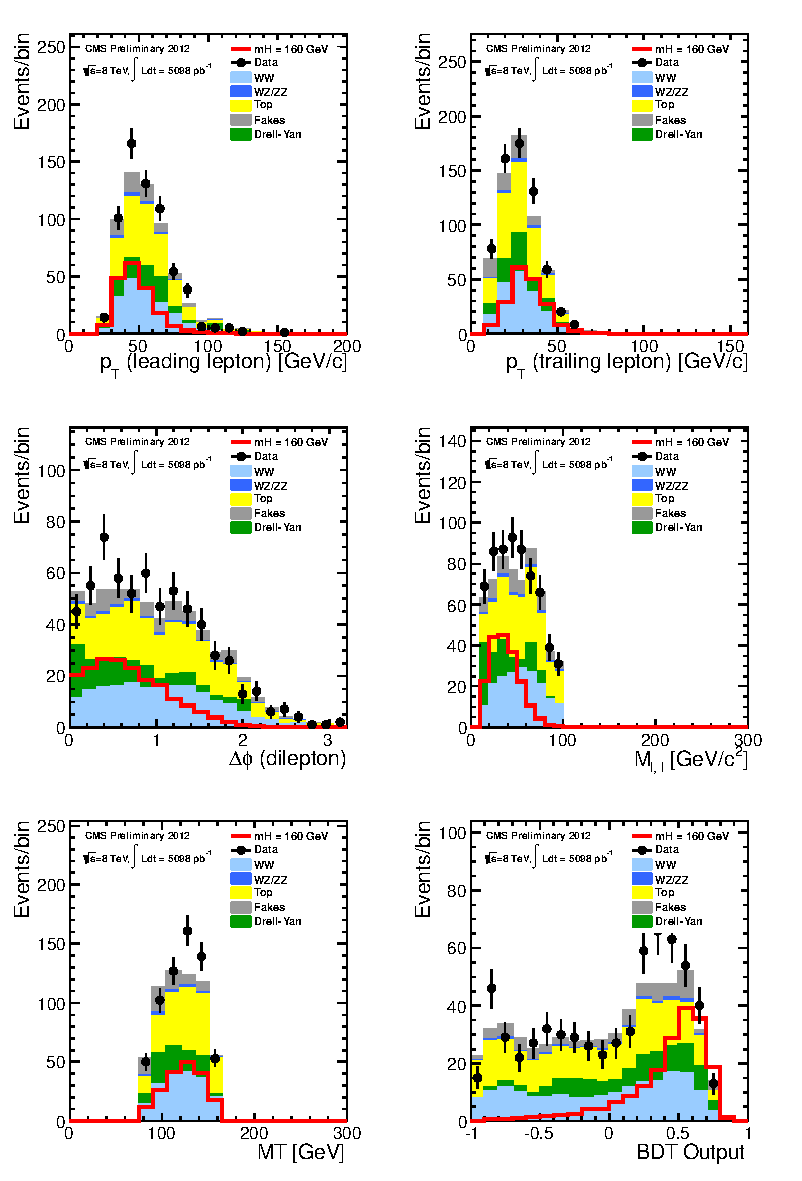
\includegraphics[width=1.0\textwidth]{figures/hww_analysis18_160_ALL_incl_1j.pdf}
\caption{Kinematic distributions in the 1-jet bin for $m_{H}=160\GeV$.}
\label{fig:hww_kinematics_160_1j}
\end{figure}
\begin{figure}[!htp]
\centering
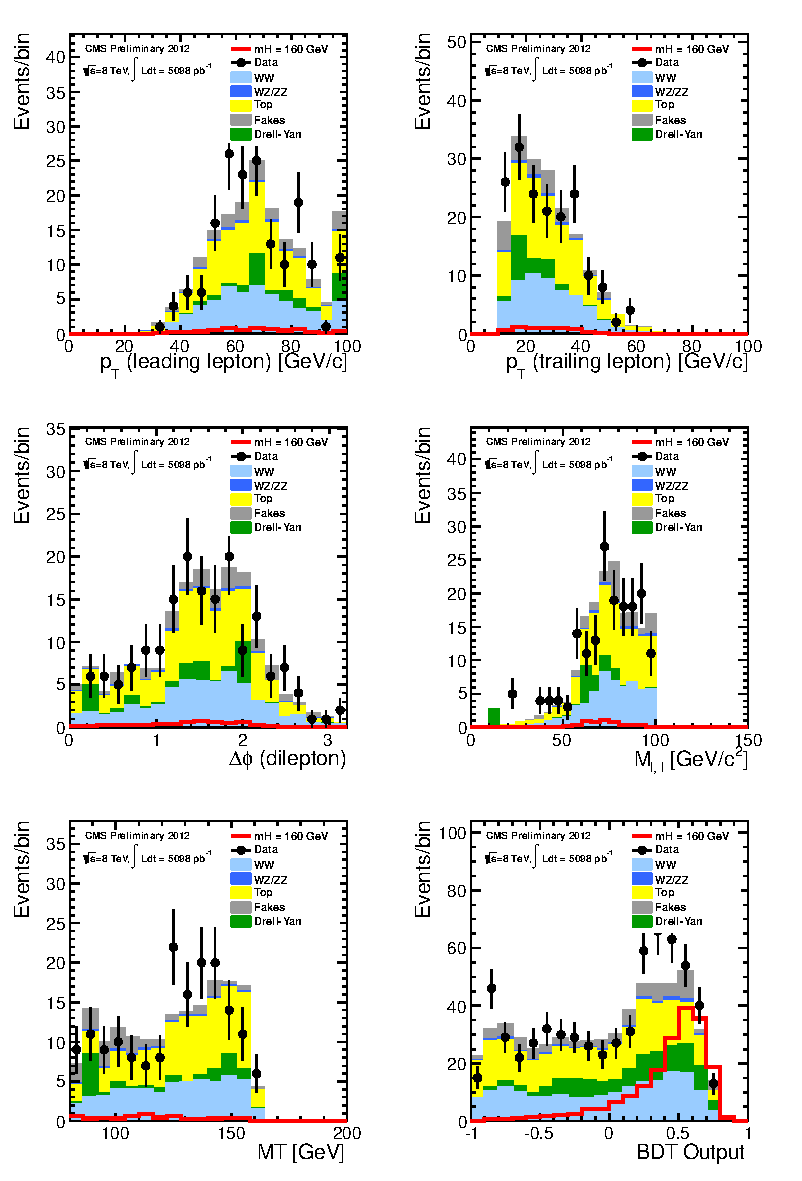
\includegraphics[width=1.0\textwidth]{figures/hww_bdtlo_analysis18_160_ALL_incl_1j.pdf}
\caption{Kinematic distributions in the 1-jet bin for $m_{H}=160\GeV$ (BDT$< -0.4$).}
\label{fig:hww_bdtlo_kinematics_160_1j}
\end{figure}
\begin{figure}[!htp]
\centering
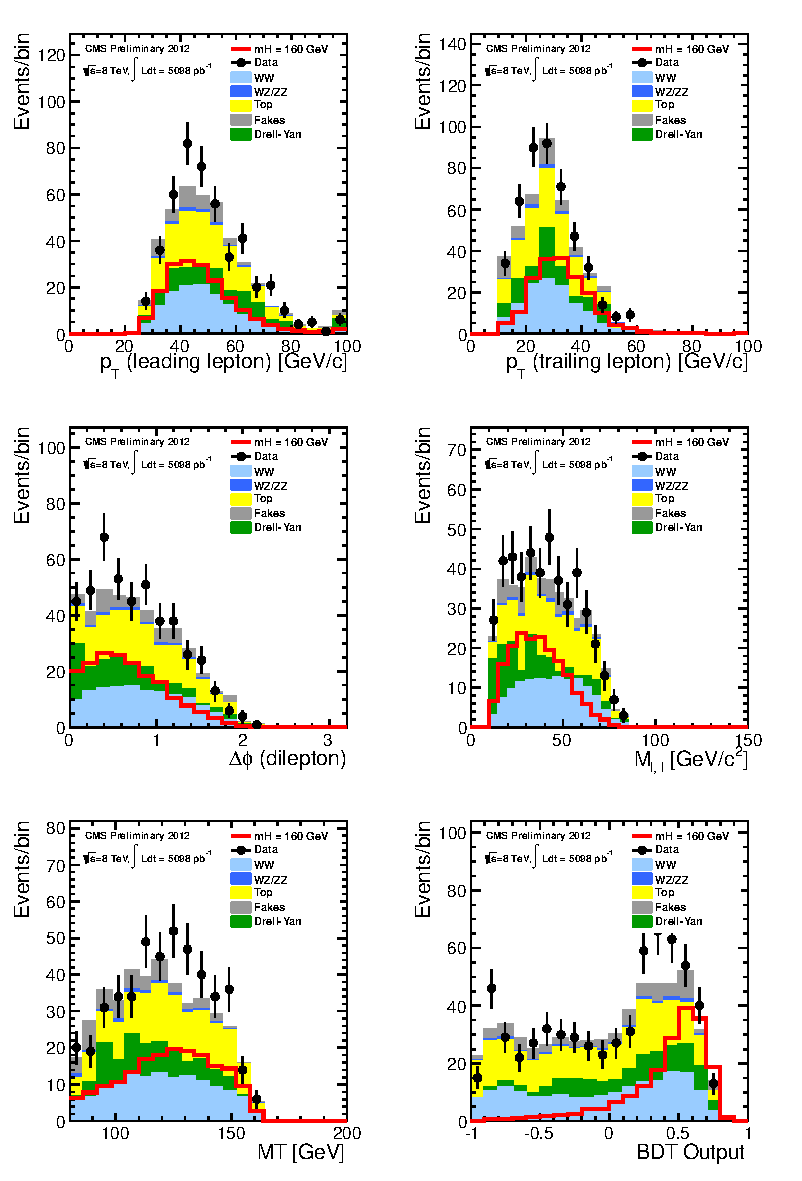
\includegraphics[width=1.0\textwidth]{figures/hww_bdthi_analysis18_160_ALL_incl_1j.pdf}
\caption{Kinematic distributions in the 1-jet bin for $m_{H}=160\GeV$ (BDT$> -0.4$).}
\label{fig:hww_bdthi_kinematics_160_1j}
\end{figure}
%%%%%%%%%%%%%%
\clearpage

%%%%%%%%%%%%%%
\begin{figure}[!htp]
\centering
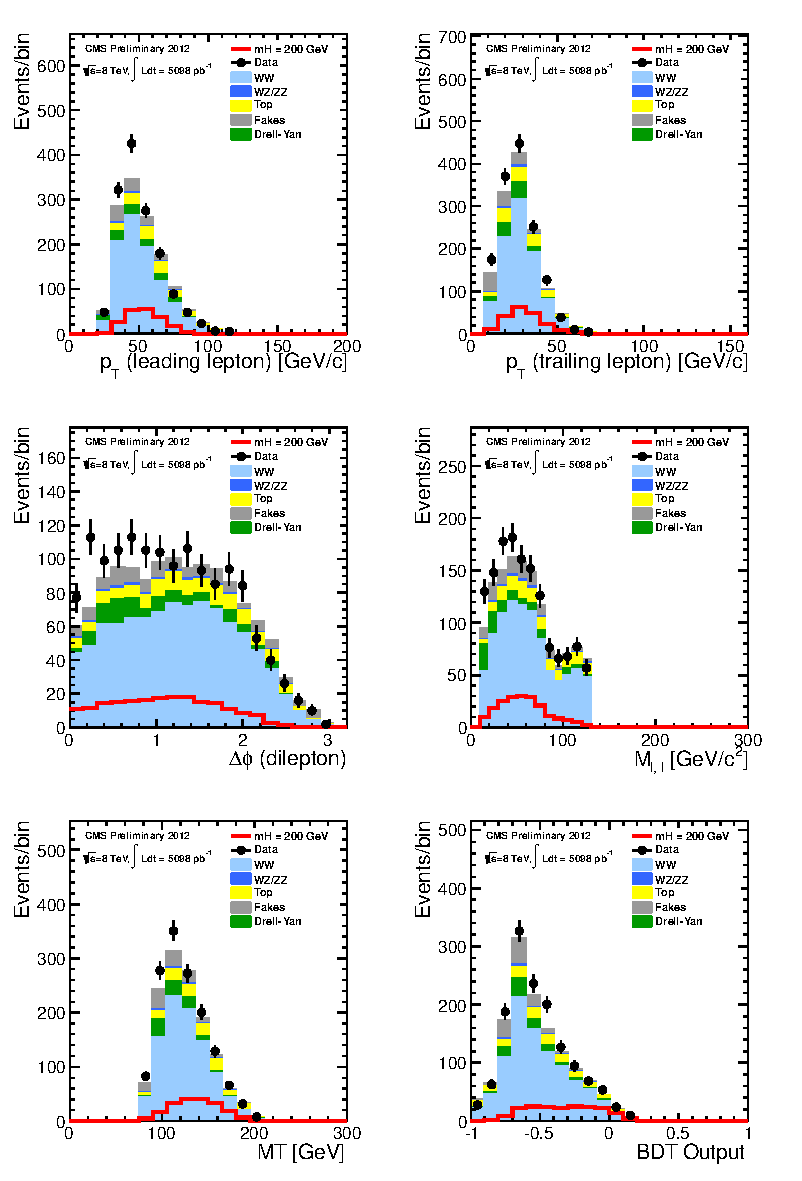
\includegraphics[width=1.0\textwidth]{figures/hww_analysis18_200_ALL_incl_0j.pdf}
\caption{Kinematic distributions in the 0-jet bin for $m_{H}=200\GeV$.}
\label{fig:hww_kinematics_200_0j}
\end{figure}
\begin{figure}[!htp]
\centering
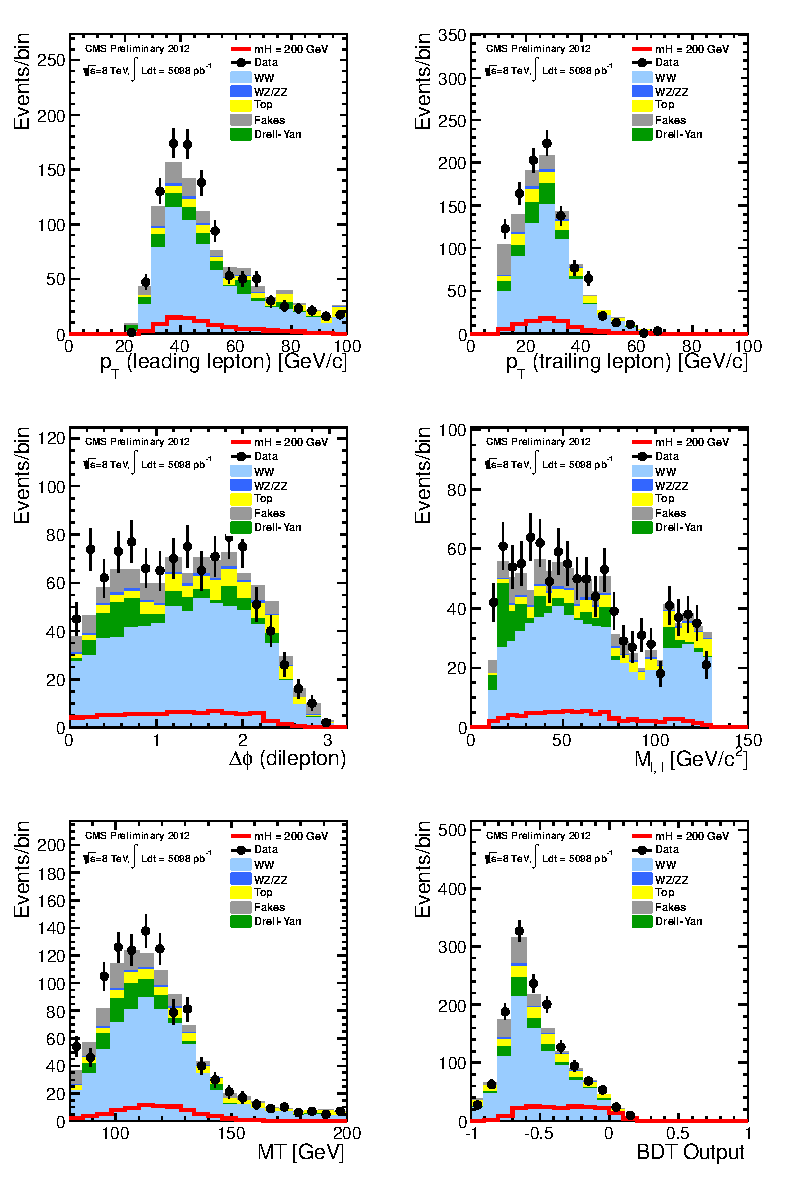
\includegraphics[width=1.0\textwidth]{figures/hww_bdtlo_analysis18_200_ALL_incl_0j.pdf}
\caption{Kinematic distributions in the 0-jet bin for $m_{H}=200\GeV$ (BDT$< -0.4$).}
\label{fig:hww_bdtlo_kinematics_200_0j}
\end{figure}
\begin{figure}[!htp]
\centering
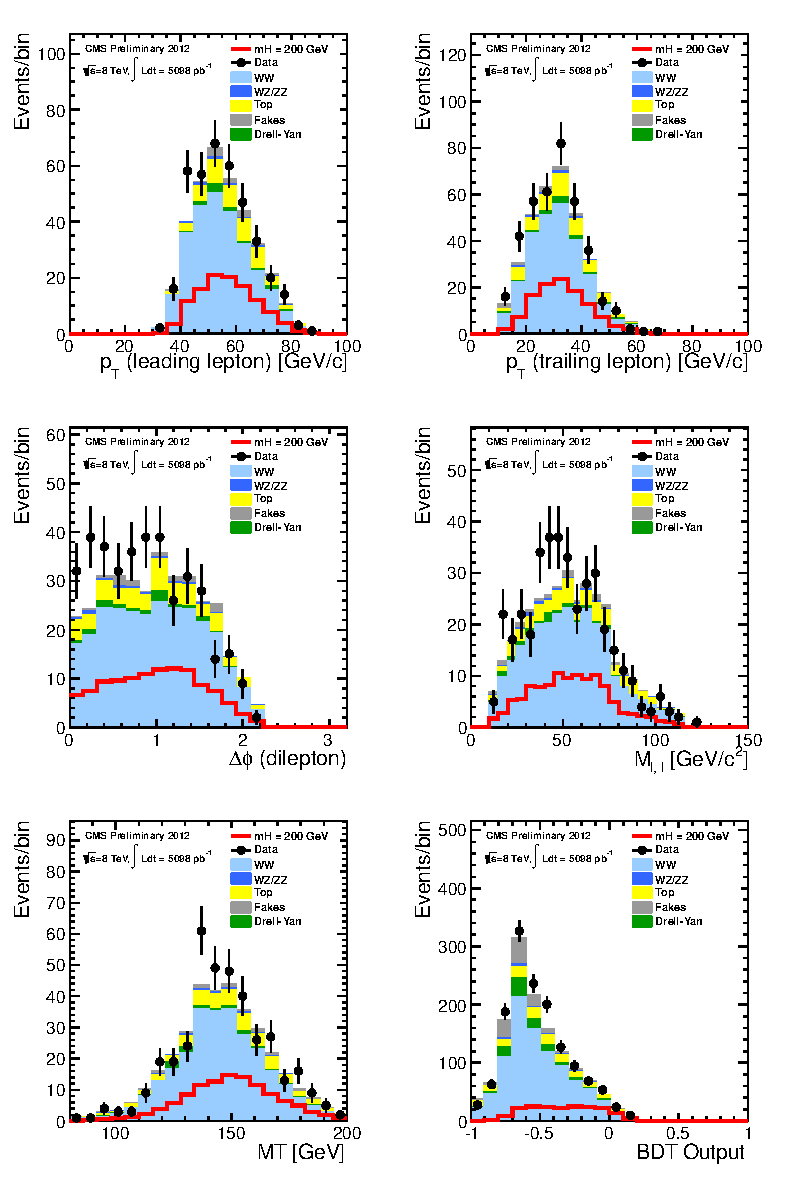
\includegraphics[width=1.0\textwidth]{figures/hww_bdthi_analysis18_200_ALL_incl_0j.pdf}
\caption{Kinematic distributions in the 0-jet bin for $m_{H}=200\GeV$ (BDT$> -0.4$).}
\label{fig:hww_bdthi_kinematics_200_0j}
\end{figure}
\begin{figure}[!htp]
\centering
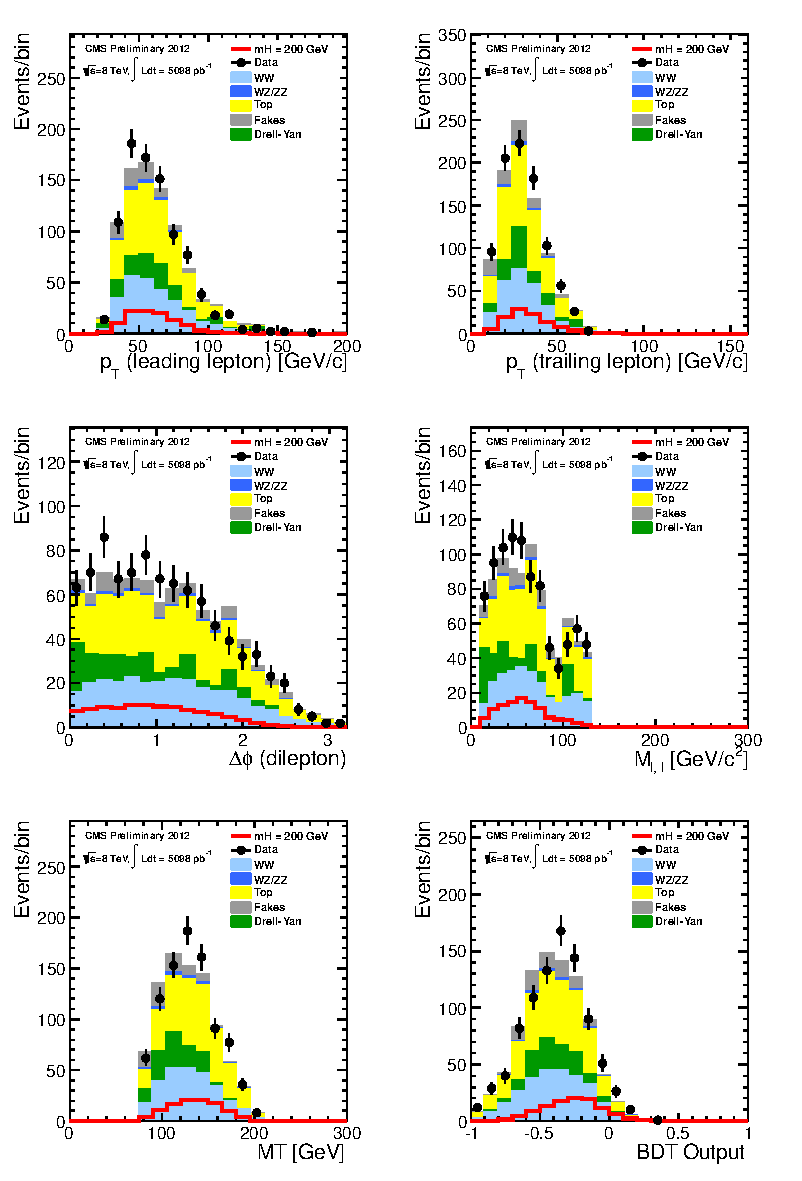
\includegraphics[width=1.0\textwidth]{figures/hww_analysis18_200_ALL_incl_1j.pdf}
\caption{Kinematic distributions in the 1-jet bin for $m_{H}=200\GeV$.}
\label{fig:hww_kinematics_200_1j}
\end{figure}
\begin{figure}[!htp]
\centering
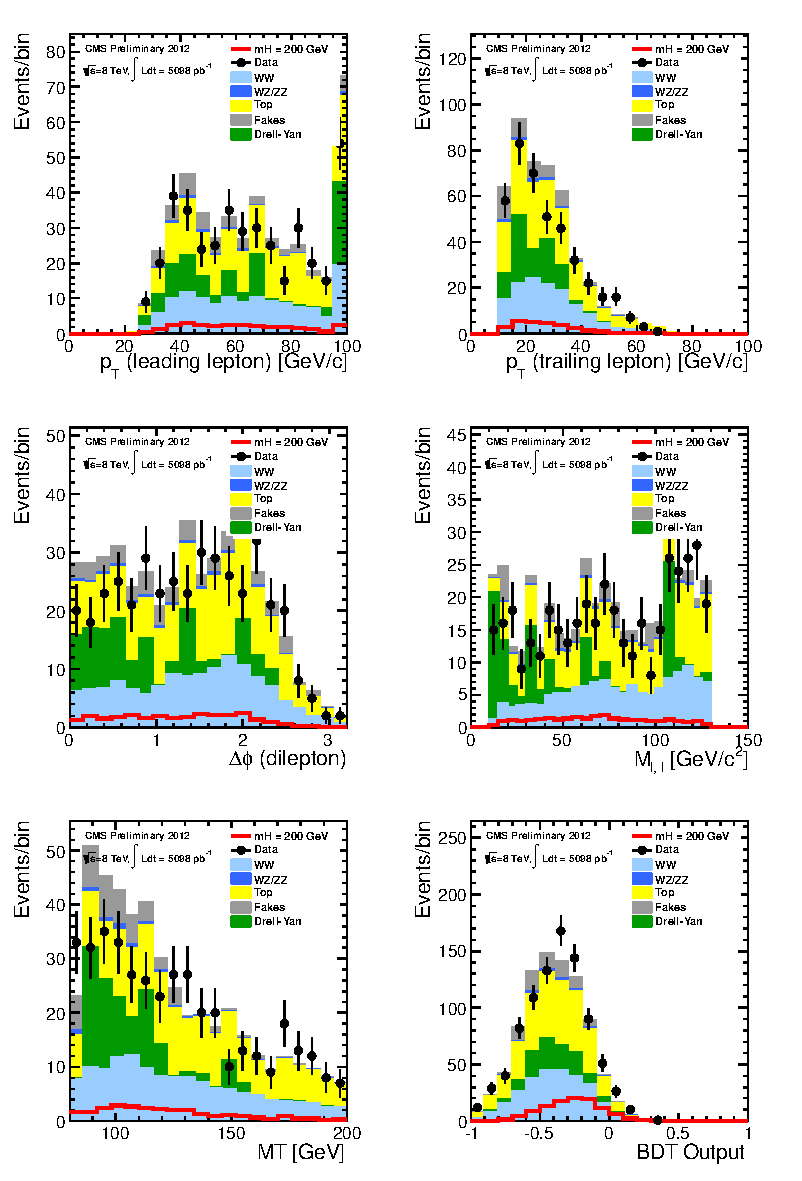
\includegraphics[width=1.0\textwidth]{figures/hww_bdtlo_analysis18_200_ALL_incl_1j.pdf}
\caption{Kinematic distributions in the 1-jet bin for $m_{H}=200\GeV$ (BDT$< -0.4$).}
\label{fig:hww_bdtlo_kinematics_200_1j}
\end{figure}
\begin{figure}[!htp]
\centering
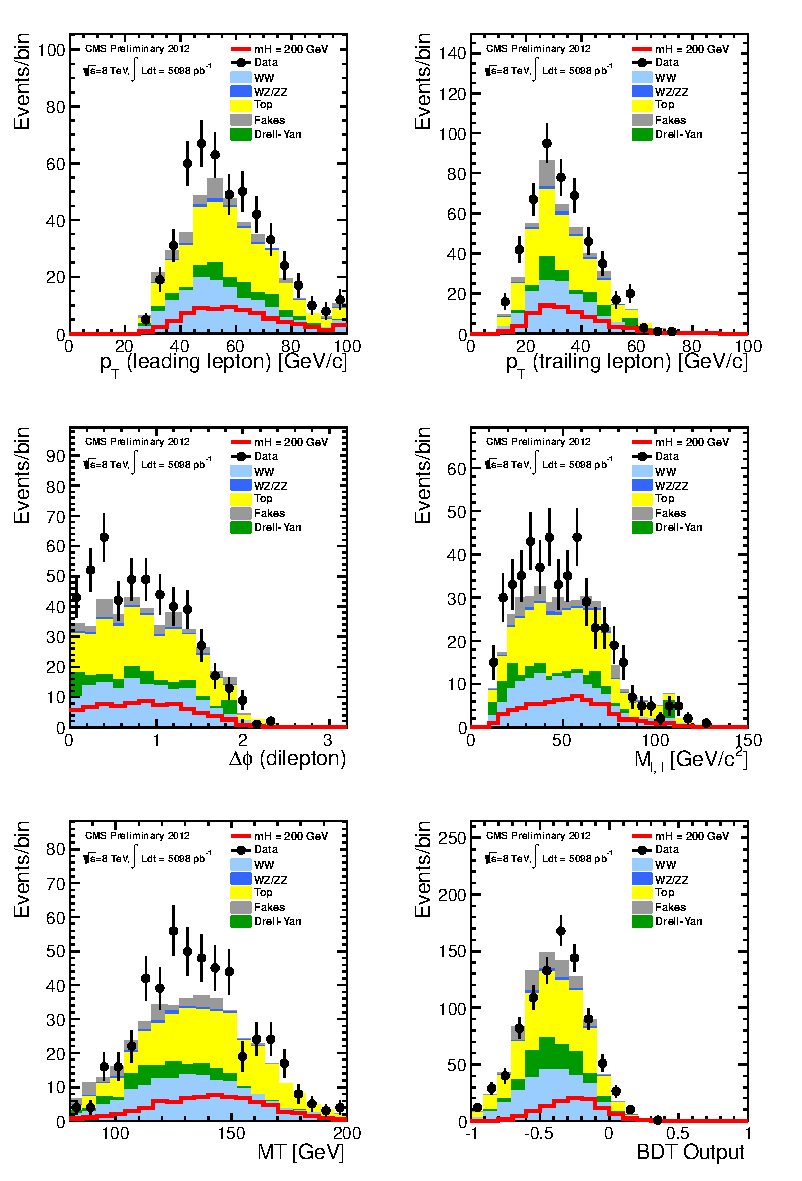
\includegraphics[width=1.0\textwidth]{figures/hww_bdthi_analysis18_200_ALL_incl_1j.pdf}
\caption{Kinematic distributions in the 1-jet bin for $m_{H}=200\GeV$ (BDT$> -0.4$).}
\label{fig:hww_bdthi_kinematics_200_1j}
\end{figure}
%%%%%%%%%%%%%%
\clearpage

